%%%%%%%%%%%%%%%%%%%%% {{{
%%Options for presentations (in-class) and handouts (e.g. print).
\documentclass[pdf,9pt]{beamer}


%%%%%%%%%%%%%%%%%%%%%%
%Change this for different slides so it appears in bar
\usepackage{authoraftertitle}
\date{Chapter 7. Linear Transformations \\ \S  7-2. Kernel and Image}

%%%%%%%%%%%%%%%%%%%%%%
%% Upload common style file
\usepackage{LyryxLAWASlidesStyle}

\begin{document}

%%%%%%%%%%%%%%%%%%%%%%%
%% Title Page and Copyright Common to All Slides

%Title Page
\input frontmatter/titlepage.tex

%LOTS Page
\input frontmatter/lyryxopentexts.tex

%Copyright Page
\input frontmatter/copyright.tex

%%%%%%%%%%%%%%%%%%%%%%%%% }}}
%-------------- start slide -------------------------------%{{{ 2

\begin{frame}[fragile]
   \tableofcontents
\end{frame}
%-------------- end slide -------------------------------%}}}
\section[\textcolor{yellow}{}]{\textcolor{yellow}{What are the Kernel and the Image?}}
%-------------- start slide -------------------------------%{{{ 3
\frame{
\frametitle{What are the Kernel and the Image?}
\pause
\begin{definition}
    Let $V$ and $W$ be vector spaces, and $T:V\rightarrow W$ a
    linear transformation.
    \begin{enumerate}
    \item The \alert{kernel} of $T$ (sometimes called the null space of $T$)
	is defined to be the set
	\[ \ker(T) = \{ \vec{v}\in V ~|~ T(\vec{v})=\vec{0}\}.\]
    \item The \alert{image} of $T$ is defined to be the set
	\[ \im(T) = \{ T(\vec{v}) ~|~ \vec{v}\in V \}.\]
    \end{enumerate}
\end{definition}
\vfill
\begin{center}
\begin{tikzpicture}[scale=0.75]
%First image
\draw (0,0) [dkgreenvect,thick] ellipse (0.95cm and 1.55cm);
\draw (3,0) [dkgreenvect,thick] ellipse (1.55cm and 0.95cm);
\draw (0,0) [dkgreenvect,thick] ellipse (0.58cm and 0.68cm);
\node[font=\footnotesize,text=white](kerT) at (0,0) {$\text{ker}(T)$};
\draw[dkgreenvect,->,thick](0.05,0.68)--(2.98,0.04);
\draw[dkgreenvect,->,thick](0.05,-0.68)--(2.98,-0.04);
\draw[-latex, dkgreenvect, thick](0.7,1.05)..controls (0.9,1.15) and (1.55,1.15)..(2.15,0.8) node[above,midway,font=\footnotesize,text=white]{$T$};
\node[font=\footnotesize,text=white] at (0,-1.15) {$V$};
\node[font=\footnotesize,text=white] at (3.5,0) {$W$};
\draw[dkgreenvect,thick] (3,0) circle (1.5pt) node[below,font=\footnotesize,text=white]{$\vec{0}$};
\end{tikzpicture}
%Second image
\qquad
\begin{tikzpicture}[scale=0.75]
\draw (0,-4) [dkgreenvect,thick] ellipse (0.95cm and 1.55cm);
\draw (3,-4) [dkgreenvect,thick] ellipse (1.55cm and 0.95cm);
\draw (2.75,-4) [dkgreenvect,thick] ellipse (0.58cm and 0.68cm);
\node[font=\footnotesize,text=white](imT) at (2.75,-4) {$\text{im}(T)$};
\node[font=\footnotesize,text=white] at (0,-4) {$V$};
\node[font=\footnotesize,text=white] at (3.95,-4) {$W$};
\draw[dkgreenvect,-latex,thick](0.95,-4)--(1.48,-4) node[above,midway,font=\footnotesize,text=white]{$T$};
\draw[dkgreenvect,->,thick](0.11,-2.46)--(2.85,-3.33);
\draw[dkgreenvect,->,thick](0.11,-5.54)--(2.85,-4.67);
\end{tikzpicture}
\end{center}

% \pause
% \vfill
% \begin{remark}
%     If $A$ is an $m\times n$ matrix and $T_A:\RR^n\to\RR^m$ is the
%     linear transformation induced by $A$, then
%     \begin{itemize}
% 	\item $\ker(T_A) = \nul(A)$;
% 	\item $\im(T_A) = \im(A)$.
%     \end{itemize}
% \end{remark}
}
%-------------- end slide -------------------------------%}}}
%-------------- start slide -------------------------------%{{{ 1
\begin{frame}[fragile]
\begin{remark}
    If $A$ is an $m\times n$ matrix and $T_A:\RR^n\to\RR^m$ is the
    linear transformation induced by $A$, then
    \begin{itemize}
	\item $\ker(T_A) = \nul(A)$;
	\item $\im(T_A) = \im(A)$.
    \end{itemize}
\end{remark}
\end{frame}
%-------------- end slide -------------------------------%}}}
%-------------- start slide -------------------------------%{{{ 4
\frame{
\begin{problem}
    Let $T:{\cal P}_1\to\RR$ be the linear transformation defined by
    \[ T(p(x))=p(1)\mbox{ for all } p(x)\in{\cal P}_1.\]
    Find $\ker(T)$ and  $\im(T)$.
\end{problem}
    \vfill
    \pause
\begin{solution}
    \begin{eqnarray*}
      \ker(T) & = & \{ p(x)\in {\cal P}_1 ~|~ p(1)=0\}                \\
              & = & \{ ax+b ~|~\forall a,b\in\RR\quad\text{and}\quad a+b=0\} \\
              & = & \{ ax-a ~|~\forall a\in\RR\}.
    \end{eqnarray*}
    \pause
    \begin{eqnarray*}
      \im(T) & = & \{ p(1) ~|~ p(x)\in {\cal P}_1 \} \\
             & = & \{ a+b ~|~ ax+b\in {\cal P}_1 \} \\
             & = & \{ a+b ~|~ \forall  a,b\in\RR \}\\
             & = & \RR.
    \end{eqnarray*}
    \myQED
\end{solution}
}
%-------------- end slide -------------------------------%}}}
%-------------- start slide -------------------------------%{{{ 5
\frame{
\begin{theorem}
    Let $V$ and $W$ be vector spaces and $T:V\to W$ a linear
    transformation.
    Then $\ker(T)$ is a subspace of $V$ and $\im(T)$ is a subspace
    of $W$.
\end{theorem}
\pause
\begin{proofnoend}[that $\ker(T)$ is a subspace of $V$]
    \begin{enumerate}
	\item Let $\vec{0}_V$ and $\vec{0}_W$ denote the zero vectors
	    of $V$ and $W$, respectively.\\
      $T$ is a linear transformation  $\Rightarrow$ $T(\vec{0}_V)=\vec{0}_W$ $\Rightarrow$ $\vec{0}_V\in\ker(T)$.
	    \pause
	\item Let $\vec{v}_1, \vec{v}_2\in \ker(T)$.
	    Then $T(\vec{v}_1)=\vec{0}$, $T(\vec{v}_2)=\vec{0}$, and
	    \[ T(\vec{v}_1+\vec{v}_2) =T(\vec{v}_1)+T(\vec{v}_2)
	    =\vec{0}+\vec{0}=\vec{0}.\]
	    Thus $\vec{v}_1+\vec{v}_2\in\ker(T)$.
	    \pause
	\item Let $\vec{v}_1\in \ker(T)$ and let $k\in\RR$.
	    Then $T(\vec{v}_1)=\vec{0}$, and
	    \[ T(k\vec{v}_1)=kT(\vec{v}_1)=k(\vec{0})=\vec{0}.\]
	    Thus $k\vec{v}_1\in\ker(T)$.
    \end{enumerate}
    \pause
    By the {\bf Subspace Test}, $\ker(T)$ is a subspace of $V$.
    \myQED
\end{proofnoend}
}
%-------------- end slide -------------------------------%}}}
%-------------- start slide -------------------------------%{{{ 6
\frame{
\begin{proofnoend}[that $\im(T)$ is a subspace of $W$]
    \begin{enumerate}
    \item Let $\vec{0}_V$ and $\vec{0}_W$ denote the zero vectors
	of $V$ and $W$, respectively.\\
	$T$ is a linear transformation  $\Rightarrow$ $T(\vec{0}_V)=\vec{0}_W$ $\Rightarrow$ $\vec{0}_W\in\im(T)$.
	\pause
    \item Let $\vec{w}_1, \vec{w}_2\in \im(T)$.
	Then there exist $\vec{v}_1,\vec{v}_2\in V$ such that
	$T(\vec{v}_1)=\vec{w}_1$, $T(\vec{v}_2)=\vec{w}_2$, and thus
	\[ \vec{w}_1+\vec{w}_2=T(\vec{v}_1)+T(\vec{v}_2) =T(\vec{v}_1+\vec{v}_2).\]
	Since $\vec{v}_1+\vec{v}_2\in V$, $\vec{w}_1+\vec{w}_2 \in \im(T)$.
	\pause
    \item Let $\vec{w}_1\in \im(V)$ and let $k\in\RR$.
	Then there exists $\vec{v}_1\in V$ such that $T(\vec{v}_1)=\vec{w}_1$, and
	\[ k\vec{w}_1=kT(\vec{v}_1)=T(k\vec{v}_1).\]
	Since $k\vec{v}_1\in V$, $k\vec{w}_1\in\im(T)$.
    \end{enumerate}
    \pause
    By the {\bf Subspace Test}, $\im(T)$ is a subspace of $W$.
    \myQED
\end{proofnoend}
}
%-------------- end slide -------------------------------%}}}
%-------------- start slide -------------------------------%{{{ 7
\frame{
\begin{definition}
    Let $V$ and $W$ be vector spaces and $T:V\to W$ a linear transformation.\\[1em]
    \begin{enumerate}
	\item The dimension of $\ker(T)$, \alert{$\dim(\ker(T))$} is called the
	    \alert{nullity} of $T$ and is denoted \alert{$\mbox{nullity}(T)$},
	    i.e.,
	    \begin{align*}
		\text{nullity}(T) = \dim(\ker(T)).
	    \end{align*}
	    \pause
	\item The dimension of $\im(T)$, \alert{$\dim(\im(T))$} is called the
	    \alert{rank} of $T$ and is denoted \alert{$\rank(T)$}, i.e.,
	    \begin{align*}
		\text{rank}(T) = \dim(\im(T)).
	    \end{align*}
    \end{enumerate}
\end{definition}
\vfill
\begin{center}
\begin{tikzpicture}[scale=0.75]
%First image
\draw (0,0) [dkgreenvect,thick] ellipse (0.95cm and 1.55cm);
\draw (3,0) [dkgreenvect,thick] ellipse (1.55cm and 0.95cm);
\filldraw (0,0) [dkgreenvect,thick] ellipse (0.58cm and 0.68cm);
\node[font=\footnotesize,text=white](kerT) at (0,0) {$\text{ker}(T)$};
\draw[dkgreenvect,->,thick](0.05,0.68)--(2.98,0.04);
\draw[dkgreenvect,->,thick](0.05,-0.68)--(2.98,-0.04);
\draw[-latex, dkgreenvect, thick](0.7,1.05)..controls (0.9,1.15) and (1.55,1.15)..(2.15,0.8) node[above,midway,font=\footnotesize,text=white]{$T$};
\node[font=\footnotesize,text=white] at (0,2) {Nullity of $T$};
\node[font=\footnotesize,text=white] at (0,-1.15) {$V$};
\node[font=\footnotesize,text=white] at (3.5,0) {$W$};
\draw[dkgreenvect,thick] (3,0) circle (1.5pt) node[below,font=\footnotesize,text=white]{$\vec{0}$};
\end{tikzpicture}
%Second image
\qquad
\begin{tikzpicture}[scale=0.75]
\draw (0,-4) [dkgreenvect,thick] ellipse (0.95cm and 1.55cm);
\draw (3,-4) [dkgreenvect,thick] ellipse (1.55cm and 0.95cm);
\filldraw (2.75,-4) [dkgreenvect,thick] ellipse (0.58cm and 0.68cm);
\node[font=\footnotesize,text=white](imT) at (2.75,-4) {$\text{im}(T)$};
\node[font=\footnotesize,text=white] at (0,-4) {$V$};
\node[font=\footnotesize,text=white] at (3.95,-4) {$W$};
\node[font=\footnotesize,text=white] at (2.85,-2) {Rank of $T$};
\draw[dkgreenvect,-latex,thick](0.95,-4)--(1.48,-4) node[above,midway,font=\footnotesize,text=white]{$T$};
\draw[dkgreenvect,->,thick](0.11,-2.46)--(2.85,-3.33);
\draw[dkgreenvect,->,thick](0.11,-5.54)--(2.85,-4.67);
\end{tikzpicture}
\end{center}
}
%-------------- end slide -------------------------------%}}}
%-------------- start slide -------------------------------%{{{ 8
\frame{
\begin{example}
    If $A$ is an $m\times n$ matrix, then $T_A:\R^n\to \R^m$ is a linear
		transformation and
    \bigskip
    \begin{minipage}{0.45 \textwidth}
    \[ \im(T_A) = \im(A) =\col(A)\]
    \[\Downarrow\]
    \begin{align*}
        \rank(T_A) &=\dim(\im(T_A))\\
                   &=\dim(\col(A))\\
                   &=\rank(A)\\
                   &= \dim(\row(A))
    \end{align*}
    \end{minipage}
    \begin{minipage}{0.5\textwidth}
        \[\ker(T_A)=\nul(A)\]
        \[\Downarrow\]
        \begin{align*}
            &\mbox{nullity}(T_A)  =\dim(\nul(A))\\
                                & =\text{``\#  of free parameters in $Ax=0$"}\\
                                & =n-\rank(A)
        \end{align*}
    \end{minipage}
    \vfill
		\[\Updownarrow\]
		\begin{align*}
				\boxed{\rank(A)+\mbox{nullity}(T_A)=\dim(\R^n)}
		\end{align*}
\end{example}
}
%-------------- end slide -------------------------------%}}}
\section[\textcolor{yellow}{}]{\textcolor{yellow}{Finding Bases of the Kernel and the Image}}
%-------------- start slide -------------------------------%{{{ 9
\frame{
\frametitle{Finding bases of the kernel and the image}
\pause
\begin{example}[continued]
    For the linear transformation $T$ defined by
    $T:{\cal P}_1\to\RR$
    \[ T(p(x))=p(1)\mbox{ for all } p(x)\in{\cal P}_1,\]
    we found that
    \begin{eqnarray*}
	\ker(T) = \{ ax-a ~|~ a\in\RR\} \quad\text{and}\quad \im(T)  = \RR.
    \end{eqnarray*}
    \pause
    \begin{itemize}
        \item $\textcolor{cyan}{\ker(T)= \Span\{(x-1)\}}$ and $\dim(\ker(T))=1=\mbox{nullity}(T)$.
            \bigskip
        \item $\textcolor{magenta}{\im(T) = \Span \{1\}}$ and $\dim(\im(T))=1=\rank(T)$
            \bigskip
        \item Hence,
            \[
                \textcolor{cyan}{\mbox{nullity}(T)} + \textcolor{magenta}{\rank(T)} = \dim(\mathcal{P}_1) = 2.
            \]
    \end{itemize}
    \myQED
    % From this, we see that ;
    % since $\{(x-1)\}$ is an independent subset of ${\cal P}_1$,
    % $\{(x-1)\}$ is a basis of $\ker(T)$.
    % Thus
    % \[ \dim(\ker(T))=1=\mbox{nullity}(T).\]
    % \pause
    % Since $\im(T)=\RR$, we can write  and
    % \[ \dim(\im(T))=1=\rank(T).\]
\end{example}
}
%-------------- end slide -------------------------------%}}}
%-------------- start slide -------------------------------%{{{ 10
\frame{
\begin{problem}
    Let $T:\bm{M}_{22}\to \bm{M}_{22}$ be defined by
    \[ T\left[\begin{array}{cc}
    a & b \\ c & d \end{array}\right]
    =
    \left[\begin{array}{cc}
    a+b & b+c \\ c+d & d+a \end{array}\right]
    \mbox{ for all }
    \left[\begin{array}{cc}
    a & b \\ c & d \end{array}\right] \in\bm{M}_{22}.\]
    Then $T$ is a linear transformation
    \alert{(you should be able to prove this).}
    Find a basis of $\ker(T)$ and a basis of $\im(T)$.
\end{problem}
\pause
\vfill
\begin{solution}
    Suppose $\left[\begin{array}{rr} a & b \\ c & d \end{array}\right]
    \in\ker(T)$.  Then
    \[
	T\left[\begin{array}{rr} a   & b   \\ c   & d \end{array}\right]
	=\left[\begin{array}{rr} a+b & b+c \\ c+d & d+a \end{array}\right]
	=\left[\begin{array}{rr} 0   & 0   \\ 0   & 0 \end{array}\right].\]
    \pause
    This gives us a system of four equations in the four variables
    $a, b, c, d$:
		\begin{align*}
			\begin{cases}
				a+b=0	\\
				b+c=0\\
				c+d=0\\
				d+a=0\\
			\end{cases}
		\end{align*}
\end{solution}
}
%-------------- end slide -------------------------------%}}}
%-------------- start slide -------------------------------%{{{ 11
\frame{
\begin{solution}[continued]
    This system has solution
    $a=-t, b=t, c=-t, d=t$ for any $t\in\RR$,
    and thus
    \[
        \ker(T)=\left\{ \left.
    \left[\begin{array}{rr} -t & t \\ -t & t \end{array}\right]
    ~\right|~ t\in\RR\right\}
    =\Span\left\{\left[\begin{array}{rr} -1 & 1 \\ -1 & 1 \end{array}\right]
    \right\}.
    \]
    \pause
    Let
		\begin{align*}
				B=\left\{\left[\begin{array}{rr} -1 & 1 \\ -1 & 1 \end{array}\right]\right\}.
		\end{align*}
    Since $B$ is an independent subset of $\bm{M}_{22}$ and $\Span(B)=\ker(T)$,
    $B$ is a basis of $\ker(T)$.
\end{solution}
}
%-------------- end slide -------------------------------%}}}
%-------------- start slide -------------------------------%{{{ 12
\frame{
\begin{solution}[continued]
		As for $\im(T)$, notice that
    \begin{eqnarray*}
	\im(T) & = & \left\{ \left.
          \left[\begin{array}{rr} \textcolor{magenta}{a}+b & b+\textcolor{red}{c} \\ \textcolor{red}{c}+\textcolor{cyan}{d} & \textcolor{cyan}{d}+\textcolor{magenta}{a} \end{array}\right]
	    ~\right|~ a,b,c,d\in\RR\right\} \\
					    & = & \Span\left\{
                    \textcolor{magenta}{\left[\begin{array}{rr} 1 & 0 \\ 0 & 1 \end{array}\right]},
                    \left[\begin{array}{rr} 1 & 1 \\ 0 & 0 \end{array}\right],
                    \textcolor{red}{\left[\begin{array}{rr} 0 & 1 \\ 1 & 0 \end{array}\right]},
                    \textcolor{cyan}{\left[\begin{array}{rr} 0 & 0 \\ 1 & 1 \end{array}\right]}
    \right\}.
	\end{eqnarray*}
	\pause

	Let
	\[ S = \left\{
		\left[\begin{array}{rr} 1 & 0 \\ 0 & 1 \end{array}\right],
		\left[\begin{array}{rr} 1 & 1 \\ 0 & 0 \end{array}\right],
		\left[\begin{array}{rr} 0 & 1 \\ 1 & 0 \end{array}\right],
		\left[\begin{array}{rr} 0 & 0 \\ 1 & 1 \end{array}\right] \right\}.\]
		\pause

    $S$ is a dependent subset of $\bm{M}_{22}$, but \alert{(check this yourselves)}
    \[ C = \left\{
	\left[\begin{array}{rr} 1 & 0 \\ 0 & 1 \end{array}\right],
	\left[\begin{array}{rr} 0 & 1 \\ 1 & 0 \end{array}\right],
    \left[\begin{array}{rr} 0 & 0 \\ 1 & 1 \end{array}\right] \right\}\]
    is an independent subset of $S$.
    Since $\Span(C)=\Span(S)=\im(T)$ and $C$ is independent, $C$ is a basis of $\im(T)$.
    \myQED
\end{solution}
}
%-------------- end slide -------------------------------%}}}
%-------------- start slide -------------------------------%{{{ 1
\begin{frame}[fragile]
   \begin{remark}
       \begin{align*}
           \dim(\bm{M}_{22}) = 4
       \end{align*}
       \begin{align*}
           \mbox{nullity}(T) =\dim(\ker(T)) = 1
       \end{align*}
       \begin{align*}
           \rank(T) = \dim(\im(T)) = 3
       \end{align*}
       \[\Downarrow\]
        \begin{align*}
            \textcolor{cyan}{\mbox{nullity}(T)} + \textcolor{magenta}{\rank(T)} = \dim(\bm{M}_{22})
        \end{align*}
   \end{remark} 
\end{frame}
%-------------- end slide -------------------------------%}}}
\section[\textcolor{yellow}{}]{\textcolor{yellow}{Surjections and Injections}}
%-------------- start slide -------------------------------%{{{ 13
\frame{
\frametitle{Surjections and Injections}
\pause
\begin{definition}
    Let $V$ and $W$ be vector spaces and $T:V\to W$ a linear
    transformation.
    \begin{enumerate}
	\item $T$ is \alert{onto} (or surjective) if $\im(T)=W$.
	\item $T$ is \alert{one-to-one} (or injective) if,
      \begin{align*}
        T(\vec{v})=T(\vec{w})  \quad\forall \vec{v}, \vec{w}\in V \qquad\Rightarrow\qquad\vec{v}=\vec{w}.
      \end{align*}
    \end{enumerate}
\end{definition}
\pause
\vfill
\begin{example}
    Let $V$ be a vector space.
    Then the identity operator on $V$, $1_V:V\to V$, is
    one-to-one and onto.
\end{example}
}
%-------------- end slide -------------------------------%}}}
%-------------- start slide -------------------------------%{{{ 14
\begin{frame}[fragile]
    \begin{center}
	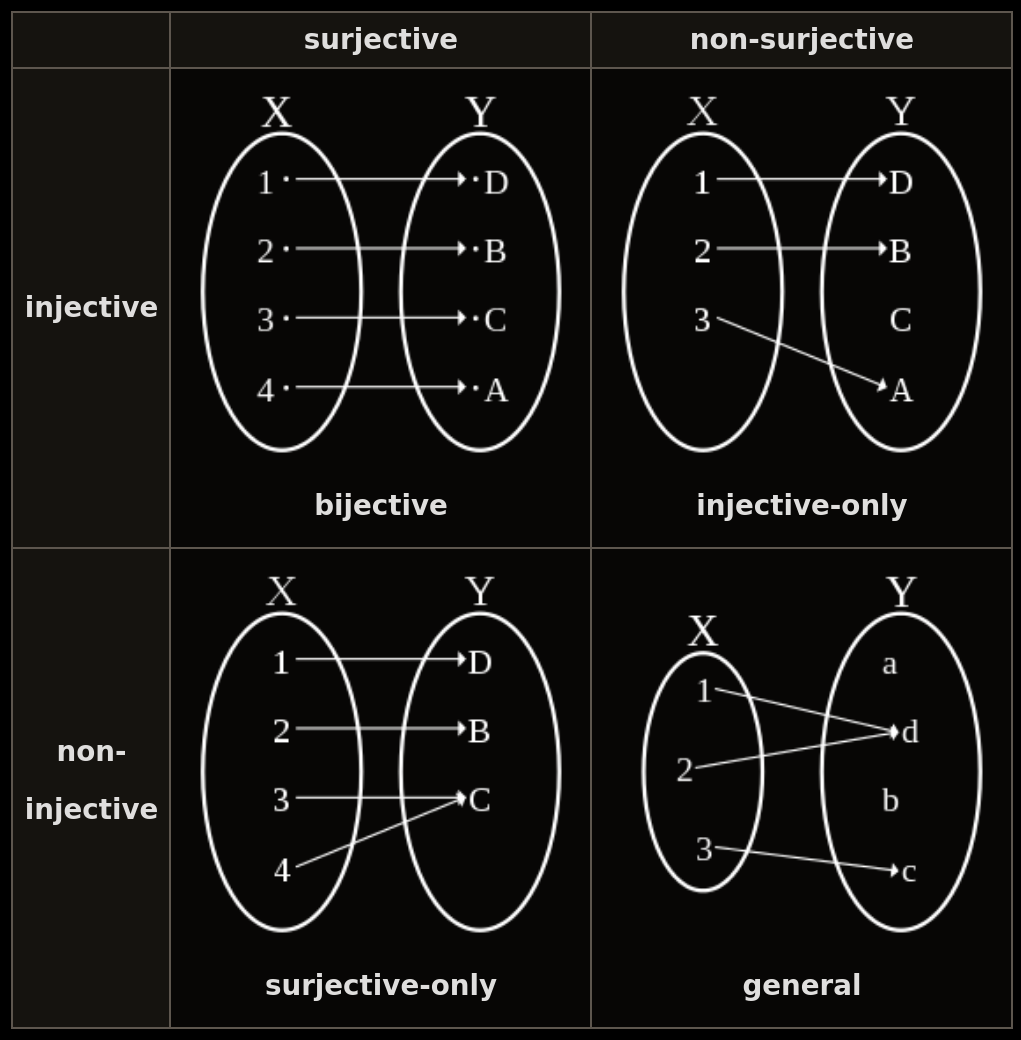
\includegraphics[scale=0.15]{./figures/Surjective-Injective-neg.png}
    \end{center}
\end{frame}
%-------------- end slide -------------------------------%}}}
%-------------- start slide -------------------------------%{{{ 15
\frame{
\begin{theorem}
    Let $V$ and $W$ be vector spaces and $T:V\to W$ a linear
    transformation.
    Then $T$ is one-to-one if and only if $\ker(T)=\{\vec{0}\}$.
\end{theorem}
\vfill
\pause
\begin{proofnoend}
    $(\Rightarrow)$
    Let $\vec{v}\in\ker(T)$.  Then
    \[ T(\vec{v})=\vec{0}=T(\vec{0}).\]
    \begin{align*}
        \text{$T$ is one-to-one} \quad \Rightarrow \quad  \vec{v}=\vec{0}\quad \Rightarrow\quad \ker T=\{\vec{0}\}
    \end{align*}
    \pause
    $(\Leftarrow)$
    Conversely, suppose that $\ker(T)=\{\vec{0}\}$,
    and let $\vec{v}, \vec{w}\in V$ be such that
    \[ T(\vec{v})=T(\vec{w}).\]
    Then $T(\vec{v})-T(\vec{w})=\vec{0}$,
    and since $T$ is a linear transformation
    \[ T(\vec{v}-\vec{w})=\vec{0}.\]
    By definition, $\vec{v}-\vec{w}\in\ker(T)$,
    implying that $\vec{v}-\vec{w}=\vec{0}$.
    Therefore $\vec{v}=\vec{w}$, and hence $T$ is one-to-one.
    \myQED
\end{proofnoend}
}
%-------------- end slide -------------------------------%}}}
%-------------- start slide -------------------------------%{{{ 16
\frame{
\begin{problem}
    Let $T:\bm{M}_{22}\to\RR^2$ be a linear transformation defined by
    \[ T\left[\begin{array}{cc}
    a & b \\ c & d \end{array}\right]
    =
    \left[\begin{array}{c}
    a+d \\ b+c \end{array}\right]
    \mbox{ for all }
    \left[\begin{array}{cc}
    a & b \\ c & d \end{array}\right] \in\bm{M}_{22}.\]
    Prove that $T$ is onto but not one-to-one.
\end{problem}
\pause
\vfill
\begin{proofnoend}
    Let $\left[\begin{array}{c} x \\ y \end{array}\right]\in\RR^2$.
    Since
    $T\left[\begin{array}{cc} x & y \\ 0 & 0 \end{array}\right]
    =\left[\begin{array}{c} x \\ y \end{array}\right]$,
    $T$  is onto.
    \bigskip

    Observe that
    $\left[\begin{array}{cc} 1 & 0 \\ 0 & -1 \end{array}\right]\in\ker(T)$,
    so $\ker(T)\neq \{\vec{0}_{22}\} $.
    By the previous  {\bf Theorem}, $T$ is not one-to-one.\myQED
\end{proofnoend}
}
%-------------- end slide -------------------------------%}}}
%-------------- start slide -------------------------------%{{{ 17
\frame{
\begin{problem}
    Suppose $U$ is an \alert{invertible} $m\times m$ matrix and
    let $T:\bm{M}_{mn}\to\bm{M}_{mn}$ be defined by
    \[ T(A)=UA\mbox{ for all } A\in\bm{M}_{mn}.\]
    Then $T$ is a linear transformation
    \textcolor{blue}{(this is left to you to verify).}
    Prove that $T$ is one-to-one and onto.
\end{problem}
\vfill
\pause
\begin{proofnoend}
    Suppose $A,B\in{\bm M}_{mn}$ and that $T(A)=T(B)$.
    Then $UA=UB$;
    since $U$ is invertible
    \begin{eqnarray*}
	U^{-1}(UA) & = & U^{-1} (UB) \\
	(U^{-1}U)A & = & (U^{-1} U)B \\
	I_{mm}A & = & I_{mm}B \\
	A & = & B.
    \end{eqnarray*}
    Therefore, $T$ is one-to-one.
\end{proofnoend}
}
%-------------- end slide -------------------------------%}}}
%-------------- start slide -------------------------------%{{{ 18
\frame{
\begin{proofnoend}[continued]
    To prove that $T$ is onto, let $B\in{\bm M}_{mn}$ and let
    $A=U^{-1}B$.
    Then
    \[ T(A)=UA=U(U^{-1}B)=(UU^{-1})B=I_{mm}B=B,\]
    and therefore $T$ is onto.
    \myQED
\end{proofnoend}
}
%-------------- end slide -------------------------------%}}}
%-------------- start slide -------------------------------%{{{ 19
\frame{
\begin{problem}
    Let $S:{\cal P}_2\to\bm{M}_{22}$ be a linear transformation
    defined by
    \[ S(ax^2+bx+c)
	=
	\left[\begin{array}{cc}
	a+b & a+c \\ b-c & b+c \end{array}\right]
	\mbox{ for all }
	ax^2+bx+c\in{\cal P}_2.\]
    Prove that $S$ is one-to-one but not onto.
\end{problem}
\pause
\vfill
\begin{proofnoend}
    By definition,
    \[ \ker(S)=\{ax^2+bx+c\in{\cal P}_2 ~|~ a+b=0,
    a+c=0, b-c=0, b+c=0\}.\]
    Suppose $p(x)=ax^2+bx+c\in\ker(S)$.
    This leads to a homogeneous system of four equations in three
    variables:
    \[ \left[\begin{array}{rrr|c}
	    1 & 1 & 0  & 0 \\
	    1 & 0 & 1  & 0 \\
	    0 & 1 & -1 & 0 \\
	    0 & 1 & 1  & 0  \end{array}\right]
    \rightarrow \cdots \rightarrow
    \left[\begin{array}{ccc|c}
	    1 & 0 & 0 & 0 \\
	    0 & 1 & 0 & 0 \\
	    0 & 0 & 1 & 0 \\
	    0 & 0 & 0 & 0  \end{array}\right]. \]
    Since the unique solution is $a=b=c=0$, $\ker(S)=\{\vec{0}\}$, and thus
    $S$ is one-to-one.
\end{proofnoend}
}
%-------------- end slide -------------------------------%}}}
%-------------- start slide -------------------------------%{{{ 20
\frame{
\begin{proofnoend}[continued]
    To show that $S$ is \alert{not} onto, show that $\im(S)\ne{\cal P}_2$;
    i.e., find a matrix $A\in\bm{M}_{22}$
    such that for \alert{every} $p(x)\in{\cal P}_2$,
    $S(p(x))\neq A$.
    Let
    \[ A=\left[\begin{array}{cc}
    0 & 1 \\ 0 & 2 \end{array}\right],\]
    and suppose $p(x)=ax^2+bx+c\in{\cal P}_2$ is such that
    $S(p(x))=A$.
    Then
    \[ \begin{array}{ll}
    a+b=0 & a+c=1 \\ b-c=0 & b+c=2 \end{array}\]
    Solving this system
    \[ \left[\begin{array}{ccc|c}
	    1 & 1 & 0  & 0 \\
	    1 & 0 & 1  & 1 \\
	    0 & 1 & -1 & 0 \\
	    0 & 1 & 1  & 2  \end{array}\right]
    \rightarrow
    \left[\begin{array}{rrr|r}
	    1         & 1          & 0          & 0         \\
	    \alert{0} & \alert{-1} & \alert{1}  & \alert{1} \\
	    \alert{0} & \alert{1}  & \alert{-1} & \alert{0} \\
	    0         & 1          & 1          & 2  \end{array}\right]. \]

    Since the system is inconsistent, there is no $p(x)\in{\cal P}_2$ so
    that $S(p(x))=A$, and therefore $S$ is not onto.\myQED
\end{proofnoend}
}
%-------------- end slide -------------------------------%}}}
%-------------- start slide -------------------------------%{{{ 21
\frame{

\begin{problem}[ One-to-one linear transformations preserve independent sets ]
    Let $V$ and $W$ be vector spaces and $T:V\to W$ a linear
    transformation.
    Prove that if $T$ is one-to-one and
    $\{\vec{v}_1, \vec{v}_2, \ldots, \vec{v}_k\}$ is an independent
    subset of $V$, then
    $\{T(\vec{v}_1), T(\vec{v}_2), \ldots, T(\vec{v}_k)\}$ is an independent
    subset of $W$.
\end{problem}
\pause
\vfill
\begin{proofnoend}
    Let $\vec{0}_V$ and $\vec{0}_W$ denote the zero vectors of $V$ and $W$,
    respectively.
    Suppose that
    \[ a_1T(\vec{v}_1) + a_2T(\vec{v}_2) +\cdots +a_kT(\vec{v}_k) =\vec{0}_W \]
    for some $a_1, a_2, \ldots, a_k\in\RR$.
    Since linear transformations preserve linear combinations (addition
    and scalar multiplication),
    \[ T(a_1\vec{v}_1 + a_2\vec{v}_2 +\cdots +a_k\vec{v}_k) =\vec{0}_W. \]
    Now, since $T$ is one-to-one, $\ker(T)=\{\vec{0}_V\}$, and thus
    \[ a_1\vec{v}_1 + a_2\vec{v}_2 +\cdots +a_k\vec{v}_k =\vec{0}_V. \]
    However, $\{\vec{v}_1, \vec{v}_2, \ldots, \vec{v}_k\}$ is independent,
    and hence $a_1=a_2=\cdots=a_k=0$.
    Therefore, $\{T(\vec{v}_1), T(\vec{v}_2), \ldots, T(\vec{v}_k)\}$
    is independent.\myQED
\end{proofnoend}
}
%-------------- end slide -------------------------------%}}}
%-------------- start slide -------------------------------%{{{ 22
\frame{
\begin{problem}[ Onto linear transformations preserve spanning sets ]
    Let $V$ and $W$ be vector spaces and $T:V\to W$ a linear
    transformation.
    Prove that if $T$ is onto and
    $V=\Span\{\vec{v}_1, \vec{v}_2, \ldots, \vec{v}_k\}$,
    then
    \[ W=\Span\{T(\vec{v}_1), T(\vec{v}_2), \ldots, T(\vec{v}_k)\}.\]
\end{problem}
\pause
\vfill
\begin{proofnoend}
    Suppose that $T$ is onto and let $\vec{w}\in W$.
    Then there exists $\vec{v}\in V$ such that $T(\vec{v})=\vec{w}$.
    Since $V=\Span\{\vec{v}_1, \vec{v}_2, \ldots, \vec{v}_k\}$, there
    exist $a_1, a_2, \ldots a_k\in\RR$ such that
    $\vec{v} = a_1\vec{v}_1 + a_2\vec{v}_2 + \cdots + a_k\vec{v}_k$.
    Since $T$ is a linear transformation,
    \begin{eqnarray*}
	\vec{w}=T(\vec{v})
    & = & T(a_1\vec{v}_1 + a_2\vec{v}_2 + \cdots + a_k\vec{v}_k) \\
    & = & a_1T(\vec{v}_1) + a_2T(\vec{v}_2) + \cdots + a_kT(\vec{v}_k),
    \end{eqnarray*}
    i.e., $\vec{w}\in\Span\{T(\vec{v}_1), T(\vec{v}_2), \ldots, T(\vec{v}_k)\}$,
    and thus
    \[ W\subseteq \Span\{T(\vec{v}_1), T(\vec{v}_2), \ldots, T(\vec{v}_k)\}.\]
    On the other hand,
    \begin{align*}
        T(\vec{v}_1), T(\vec{v}_2), \ldots, T(\vec{v}_k)\in W
        \quad\Longrightarrow\quad
        \Span\{T(\vec{v}_1), T(\vec{v}_2), \ldots, T(\vec{v}_k)\}\subseteq W.
    \end{align*}
    Therefore, $W=\Span\{T(\vec{v}_1), T(\vec{v}_2), \ldots, T(\vec{v}_k)\}$.
    \myQED
\end{proofnoend}
}
%-------------- end slide -------------------------------%}}}
%-------------- start slide -------------------------------%{{{ 23
\frame{
\begin{emptytitle}
Suppose $A$ is an $m\times n$ matrix.
How do we determine if $T_A:\RR^n\to\RR^m$ is onto?
How do we determine if $T_A:\RR^n\to\RR^m$ is one-to-one?
\end{emptytitle}
\pause
\begin{theorem}
Let $A$ be an $m\times n$ matrix, and
$T_A:\RR^n\to\RR^m$ the linear transformation induced by $A$.
\begin{enumerate}
    \item $T_A$ is onto if and only if $\rank(A)=m$.
    \item $T_A$ is one-to-one if and only if $\rank(A)=n$.
\end{enumerate}
\end{theorem}
\pause
\vfill
\begin{proofnoend}[sketch]
    \begin{enumerate}
	\item $T_A$ is onto if and only if $\im(T_A)=\RR^m$.
	    This is equivalent to $\col(A)=\RR^m$,
	    which occurs if and only if $\dim(\col(A))=m$,
	    i.e., $\rank(A)=m$.
	\item $\ker(T_A)=\nul(A)$, and $\nul(A)=\{\vec{0}\}$ if and only if
	    $A\vec{x}=\vec{0}$ has the \alert{unique} solution $\vec{x}=\vec{0}$.
	    Thus and row echelon form of $A$ has a leading one in every column,
	    which occurs if and only if $\rank(A)=n$. \myQED
    \end{enumerate}
\end{proofnoend}
}
%-------------- end slide -------------------------------%}}}
\section[\textcolor{yellow}{}]{\textcolor{yellow}{The Dimension Theorem (Rank-Nullity Theorem)}}
%-------------- start slide -------------------------------%{{{ 24
\frame{
\frametitle{The Dimension Theorem (Rank-Nullity Theorem)}
\pause
\begin{emptytitle}
    Suppose $A$ is an $m\times n$ matrix with rank $r$.
    Since $\im(T_A)=\col(A)$,
    \[ \dim(\im(T_A))=\rank(A)=r.\]
    We also know that $\ker(T_A)=\nul(A)$, and that
    $\dim(\nul(A))=n-r$.
    Thus,
    \[ \dim(\im(T_A)) +\dim(\ker(T_A)) = n=\dim~\RR^n.\]
\end{emptytitle}
\pause
\vfill
\begin{theorem}[Dimension Theorem (Rank-Nullity Theorem)]
    Let $V$ and $W$ be vector spaces and $T:V\to W$ a linear
    transformation.
    If $\ker(T)$ and $\im(T)$ are both finite dimensional,
    then $V$ is finite dimensional,
    and
    \[ \dim(V) = \dim(\ker(T)) + \dim(\im(T)).\]
    Equivalently, $\dim(V) = \mbox{nullity}(T) + \rank(T)$.
\end{theorem}
}
%-------------- end slide -------------------------------%}}}
%-------------- start slide -------------------------------%{{{ 25
\begin{frame}[fragile]
   \begin{center}
       
\includegraphics[scale=0.08]{./figures/Rank-nullity.png}
   \end{center}
\end{frame}
%-------------- end slide -------------------------------%}}}
%-------------- start slide -------------------------------%{{{ 1
\begin{frame}[fragile]
\begin{center}
\begin{tikzpicture}[scale=0.75]
%First image
\draw (0,0) [dkgreenvect,thick] ellipse (0.95cm and 1.55cm);
\draw (3,0) [dkgreenvect,thick] ellipse (1.55cm and 0.95cm);
\filldraw (0,0) [dkgreenvect,thick] ellipse (0.58cm and 0.68cm);
\node[font=\footnotesize,text=white](kerT) at (0,0) {$\text{ker}(T)$};
\draw[dkgreenvect,->,thick](0.05,0.68)--(2.98,0.04);
\draw[dkgreenvect,->,thick](0.05,-0.68)--(2.98,-0.04);
\draw[-latex, dkgreenvect, thick](0.7,1.05)..controls (0.9,1.15) and (1.55,1.15)..(2.15,0.8) node[above,midway,font=\footnotesize,text=white]{$T$};
\node[font=\footnotesize,text=white] at (0,-1.15) {$V$};
\node[font=\footnotesize,text=white] at (3.5,0) {$W$};
\draw[dkgreenvect,thick] (3,0) circle (1.5pt) node[below,font=\footnotesize,text=white]{$\vec{0}$};
\end{tikzpicture}
%Second image
\quad $+$\quad
\begin{tikzpicture}[scale=0.75]
\draw (0,-4) [dkgreenvect,thick] ellipse (0.95cm and 1.55cm);
\draw (3,-4) [dkgreenvect,thick] ellipse (1.55cm and 0.95cm);
\filldraw (2.75,-4) [dkgreenvect,thick] ellipse (0.58cm and 0.68cm);
\node[font=\footnotesize,text=white](imT) at (2.75,-4) {$\text{im}(T)$};
\node[font=\footnotesize,text=white] at (0,-4) {$V$};
\node[font=\footnotesize,text=white] at (3.95,-4) {$W$};
\draw[dkgreenvect,-latex,thick](0.95,-4)--(1.48,-4) node[above,midway,font=\footnotesize,text=white]{$T$};
\draw[dkgreenvect,->,thick](0.11,-2.46)--(2.85,-3.33);
\draw[dkgreenvect,->,thick](0.11,-5.54)--(2.85,-4.67);
\end{tikzpicture}

\[||\]

\begin{tikzpicture}[scale=0.75]
		\filldraw (0,-4) [dkgreenvect,thick] ellipse (0.95cm and 1.55cm);
		\node[font=\footnotesize,text=white] at (0,-4) {$V$};
\end{tikzpicture}
\end{center}
\end{frame}
%-------------- end slide -------------------------------%}}}
%-------------- start slide -------------------------------%{{{ 26
\frame{
\begin{proofnoend}[Outline]
    Let $\vec{w}\in\im(T)$;
    then $\vec{w}=T(\vec{v})$ for some $\vec{v}\in V$.
    Suppose
    \[ \left\{ T(\vec{b}_1), T(\vec{b}_2), \ldots, T(\vec{b}_r)\right\}\]
    is a basis of $\im(T)$,
    and that
    \[ \left\{ \vec{f}_1, \vec{f}_2, \ldots, \vec{f}_k\right\}\]
    is a basis of $\ker(T)$.
    We define
    \[ B=\left\{ \vec{b}_1, \vec{b}_2, \ldots, \vec{b}_r,
    \vec{f}_1, \vec{f}_2, \ldots, \vec{f}_k\right\}.\]
    \alert{To prove that $B$ is a basis of $V$, it remains
    to prove that $B$ spans $V$ and that $B$ is linearly independent.}
    \medskip

    Since $B$ is independent and spans $V$, $B$ is a basis of $V$,
    implying $V$ is finite dimensional ($V$ is spanned by a finite set
    of vectors).
    Furthermore, $|B|=r+k$,
    so
    \[ \dim(V) = \dim(\im(T)) + \dim(\ker(T)).\]
    \myQED
\end{proofnoend}
}
%-------------- end slide -------------------------------%}}}
%-------------- start slide -------------------------------%{{{ 27
\frame{
\begin{remark}
\begin{enumerate}
    \item It is not an assumption of the theorem that $V$ is
	finite dimensional.
	Rather, it is a consequence of the assumption that both
	$\im(T)$ and $\ker(T)$ are finite dimensional.
	\pause
    \item
	As a consequence of the {\bf Dimension Theorem}, if $V$ is a finite
	dimensional vector space and either $\dim(\ker(T))$ or
	$\dim(\im(T))$ is known, then the other can be easily found.
\end{enumerate}
\end{remark}
\pause
\vfill
\begin{example}
Let $V$ and $W$ be vector spaces and $T:V\to W$ a linear
transformation.
If $V$ is finite dimensional, then it follows that
\[ \dim(\ker(T))\leq\dim(V)\quad\text{and}\quad
\dim(\im(T))\leq\dim(V).\]
\end{example}
}
%-------------- end slide -------------------------------%}}}
%-------------- start slide -------------------------------%{{{ 28
\frame{
\begin{problem}
    For $a\in\RR$, recall that the linear transformation
    $E_a:{\cal P}_n\to\RR$,
    the evaluation map at $a$, is defined as
    \[ E_a(p(x)) = p(a) \mbox{ for all } p(x)\in{\cal P}_n.\]
    Prove that $E_a$ is onto, and that
    \[ B=\{ (x-a), (x-a)^2, (x-a)^3, \ldots, (x-a)^n\}\]
    is a basis of $\ker(E_a)$.
\end{problem}
}
%-------------- end slide -------------------------------%}}}
%-------------- start slide -------------------------------%{{{ 29
\frame{
\begin{proofnoend}
    Let $t\in\RR$, and choose $p(x)=t\in{\cal P}_n$.
    Then $p(a)=t$, so $E_a(p(x))=t$, i.e., $E_a$ is onto.
    \bigskip
    \pause

    By the {\bf Dimension Theorem},
    \[ n+1=\dim({\cal P}_n) = \dim(\ker(E_a)) + \dim(\im(E_a)).\]
    Since $E_a$ is onto, $\dim(\im(E_a))=\dim(\RR) =1$,
    and thus $\dim(\ker(E_a))=n$.
    \bigskip
    \pause

    It now suffices to find $n$ independent polynomials in $\ker(E_a)$.
    \bigskip
    \pause

    Note that $(x-a)^j\in\ker(E_a)$ for $j=1,2, \ldots, n$, so
    $B\subseteq \ker(E_a)$.
    \bigskip
    \pause

    Furthermore, $B$ is independent because the polynomials in $B$
    have distinct degrees.
    \bigskip
    \pause

    Since $|B|=n=\dim(\ker(E_a))$, $B$ spans $\ker(E_a)$.
    \bigskip
    \pause

    Therefore, $B$ is a basis of  $\ker(E_a)$.
    \myQED
\end{proofnoend}
}
%-------------- end slide -------------------------------%}}}
%-------------- start slide -------------------------------%{{{ 30
\frame{
\begin{theorem}
    Let $V$ and $W$ be vector spaces, $T:V\to W$ a linear
    transformation, and
    \[ B=\left\{
	    \vec{b}_1, \vec{b}_2, \ldots, \vec{b}_r,
    \vec{b}_{r+1}, \vec{b}_{r+2}, \ldots, \vec{b}_n\right\}\]
    a basis of $V$ with the property that
    $\left\{ \vec{b}_{r+1}, \vec{b}_{r+2}, \ldots, \vec{b}_n\right\}$
    is a basis of $\ker(T)$.
    Then
    \[\left\{ T(\vec{b}_1), T(\vec{b}_2), \ldots, T(\vec{b}_r) \right\} \]
    is a basis of $\im(T)$, and therefore $r=\rank(T)$.
\end{theorem}
\pause
\vfill
\begin{remark}[ How is this useful? ]
    Suppose $V$ and $W$ are vector spaces and $T:V\to W$ is a linear
    transformation.
    If you find a basis of $\ker(T)$, then this may be used to find
    a basis of $\im(T)$:
    extend the basis of $\ker(T)$ to a basis of $V$;
    applying the transformation $T$ to each of the vectors that
    was added to the basis of $\ker(T)$ produces a set of vectors
    that is a basis of $\im(T)$.
\end{remark}
}
%-------------- end slide -------------------------------%}}}
%-------------- start slide -------------------------------%{{{ 31
\frame{
\begin{problem}
    Let
    $A=\left[\begin{array}{cc} 0 & 1 \\ 1 & 0 \end{array}\right]$,
    and let $T:\bm{M}_{22}\to\bm{M}_{22}$ be a linear transformation
    defined by
    \[ T(X)=XA-AX\mbox{ for all } X\in\bm{M}_{22}.\]
    Find a basis of $\ker(T)$ and a basis of $\im(T)$.
\end{problem}
\pause
\vfill
\begin{solution}
    First note that by the {\em Dimension Theorem},
    \[ \dim(\ker(T))+\dim(\im(T))=\dim(\bm{M}_{22})=4.\]
    Let
    $X=\left[\begin{array}{cc} a & b \\ c & d \end{array}\right]$.
    Then
    \begin{eqnarray*}
	T(X) & = & AX-XA \\
	     & = & \left[\begin{array}{cc} 0 & 1 \\ 1 & 0 \end{array}\right]
	\left[\begin{array}{cc} a  & b \\ c & d \end{array}\right]
	-\left[\begin{array}{cc} a & b \\ c & d \end{array}\right]
	\left[\begin{array}{cc} 0  & 1 \\ 1 & 0 \end{array}\right] \\
	     & = & \left[\begin{array}{cc} c & d \\ a & b \end{array}\right]
	-\left[\begin{array}{cc} b & a \\ d & c  \end{array}\right]
	= \left[\begin{array}{cc} c-b & d-a \\ a-d & b-c \end{array}\right]
    \end{eqnarray*}
\end{solution}
}
%-------------- end slide -------------------------------%}}}
%-------------- start slide -------------------------------%{{{ 32
\frame{
\begin{solution}[continued]
    If $X\in\ker(T)$, then $T(X)=\vec{0}_{22}$ so
    \begin{align*}
        \begin{cases}
        c-b=0\\ d-a=0\\ a-d=0\\ b-c=0
        \end{cases}
        \qquad
        \Longrightarrow
        \qquad
        \begin{cases}
            a=s\\ b=t\\ c=t\\ d=s
        \end{cases}
        \qquad\text{for $s,t\in\RR$.}
    \end{align*}
    Therefore,
    \[ \ker(T)=\left\{ \left.
		\left[\begin{array}{cc} s & t \\ t & s \end{array}\right]
	    ~\right|~ s,t\in\RR\right\}
	    =\Span\left\{
		\left[\begin{array}{cc} 1 & 0 \\ 0 & 1 \end{array}\right],
		\left[\begin{array}{cc} 0 & 1 \\ 1 & 0 \end{array}\right] \right\}.  \]
	    Let
    \begin{align*}
        B=\left\{
          \left[\begin{array}{cc} 1 & 0 \\ 0 & 1 \end{array}\right],
          \left[\begin{array}{cc} 0 & 1 \\ 1 & 0 \end{array}\right] \right\}
    \end{align*}
    Since $B$ is independent and spans $\ker(T)$, $B_k$ is a basis of $\ker(T)$.
\end{solution}
}
%-------------- end slide -------------------------------%}}}
%-------------- start slide -------------------------------%{{{ 33
\frame{
\begin{solution}[continued]
	To find a basis of $\im(T)$, extend the basis of $\ker(T)$ to a basis
	of $\bm{M}_{22}$: here is one such basis
	\[ \left\{
		\left[\begin{array}{cc} 1 & 0 \\ 0 & 1 \end{array}\right],
		\left[\begin{array}{cc} 0 & 1 \\ 1 & 0 \end{array}\right],
		\textcolor{magenta}{\left[\begin{array}{cc} 1 & 0 \\ 0 & 0 \end{array}\right]},
		\textcolor{yellow}{\left[\begin{array}{cc} 0 & 1 \\ 0 & 0 \end{array}\right]}
    \right\}.\]
    Therefore,
    \[ C=\left\{
      T\textcolor{magenta}{\left[\begin{array}{cc} 1 & 0 \\ 0 & 0 \end{array}\right]},
      T\textcolor{yellow}{\left[\begin{array}{cc} 0 & 1 \\ 0 & 0 \end{array}\right]}
      \right\}
      = \left\{
        \left[\begin{array}{cc} 0 & -1 \\ 1 & 0 \end{array}\right],
        \left[\begin{array}{cc} -1 & 0 \\ 0 & 1 \end{array}\right]\right\} \]
    is a basis of $\im(T)$.
    \myQED
\end{solution}
}
%-------------- end slide -------------------------------%}}}
\end{document}
